\documentclass{beamer}
\usetheme{metropolis}
\title{Global Non-Determinism With Termination}
\date{\today}
\author{Pepijn Kokke}
\institute{University of Edinburgh}
\usepackage{cmap}
\usepackage{alphabeta}
\usepackage[greek,english]{babel}
\languageattribute{greek}{polutoniko}
\usepackage{hyperref}
\usepackage{comment}
\usepackage{lmodern}

%%% TikZ and QTree

\usepackage{tikz}
\usepackage{tikz-qtree}

%%% Term Language
\newcommand{\subst}[3]{\ensuremath{#1 \{ #2 / #3 \}}}
\newcommand{\case}[3]{%
\toks0={#2#3}%
\edef\param{\the\toks0}%
\ifx\param\empty
  \ensuremath{\text{case} \; #1 \; \{\}}
\else
  \ensuremath{\text{case} \; #1 \; \{ #2 ; #3 \}}
\fi}
\newcommand{\inl}[2]{%
  \ensuremath{#1[\text{inl}].#2}}
\newcommand{\inr}[2]{%
  \ensuremath{#1[\text{inr}].#2}}

%%% Local Variables:
%%% TeX-master: "main"
%%% End:
\begin{document}

\maketitle

\begin{frame}{This is how I write \textpi-calculus things}
  \[\!
    \begin{aligned}
      P, Q ::=&\;\nu x.P        &&\text{create a new channel $x$}
      \\  \mid&\;x[y].P         &&\text{send a channel $y$ over $x$, then run P}
      \\  \mid&\;x(y).P         &&\text{receive a channel $y$ over $x$, then run P}
      \\  \mid&\;0              &&\text{halt}
      \\  \mid&\;\inl{x}P       &&\text{send a bit (inl) over $x$, then run P}
      \\  \mid&\;\inr{x}P       &&\text{send a bit (inr) over $x$, then run P}
      \\  \mid&\;\case{x}{P}{Q} &&\text{receive a bit over $x$, then run P or Q}
      \\  \mid&\;x[].P          &&\text{send a ping over $x$, then run P}
      \\  \mid&\;x().P          &&\text{receive a ping over $x$, then run P}
      \\  \mid&\;\case{x}{}{}   &&\text{loop}\]
  \end{aligned}
  
\end{frame}

\begin{frame}{Local choice}
  \centering
  \begin{tikzpicture}[sibling distance=3cm,level distance=3cm]
    \Tree
    [.{$P + Q$} \edge[->]; {$P$} \edge[->]; {$Q$} ]
  \end{tikzpicture}
\end{frame}

\begin{frame}{Non-determinism in the \textpi-calculus}
  \centering
  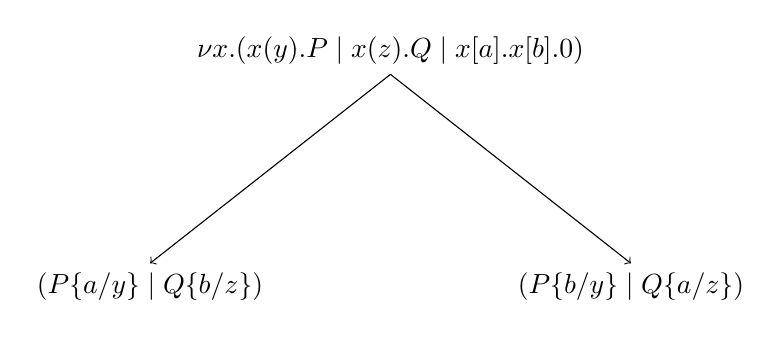
\begin{tikzpicture}[sibling distance=3cm,level distance=3cm]
    \Tree
    [.{$\nu x.(x(y).P \mid x(z).Q \mid x[a].x[b].0)$}
    \edge[->]; {$(\subst{P}{a}{y} \mid \subst{Q}{b}{z})$}
    \edge[->]; {$(\subst{P}{b}{y} \mid \subst{Q}{a}{z})$}
    ]
  \end{tikzpicture}
\end{frame}

\begin{frame}{``Local'' choice in the \textpi-calculus}
  \centering
  \only<1>{%
    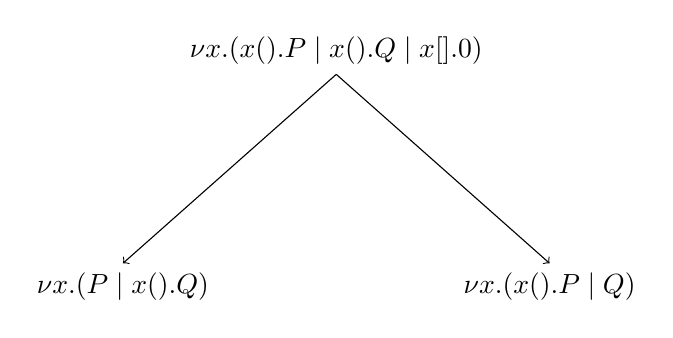
\begin{tikzpicture}[sibling distance=3cm,level distance=3cm]
      \Tree
      [.{$\nu x.(x().P \mid x().Q \mid x[].0)$}
      \edge[->]; {$\nu x.(P \mid x().Q)$}
      \edge[->]; {$\nu x.(x().P \mid Q)$}
      ]
    \end{tikzpicture}
  }
  \only<2>{%
    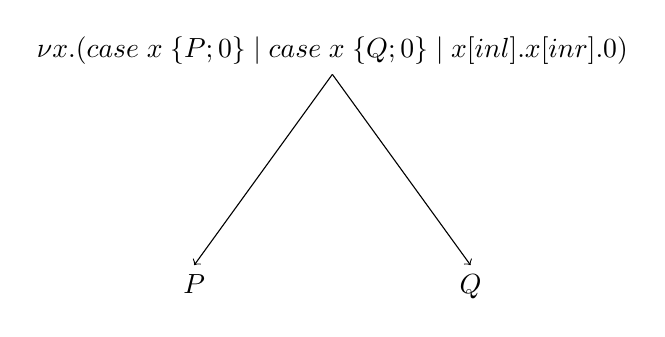
\begin{tikzpicture}[sibling distance=3cm,level distance=3cm]
      \Tree
      [.{$\nu x.(\case{x}{P}{0} \mid \case{x}{Q}{0} \mid \inl{x}\inr{x}{0})$}
      \edge[->]; {$P$}
      \edge[->]; {$Q$}
      ]
    \end{tikzpicture}
  }
\end{frame}

\begin{frame}{Non-determinism in the \textpi-calculus using local choice}
  \centering
  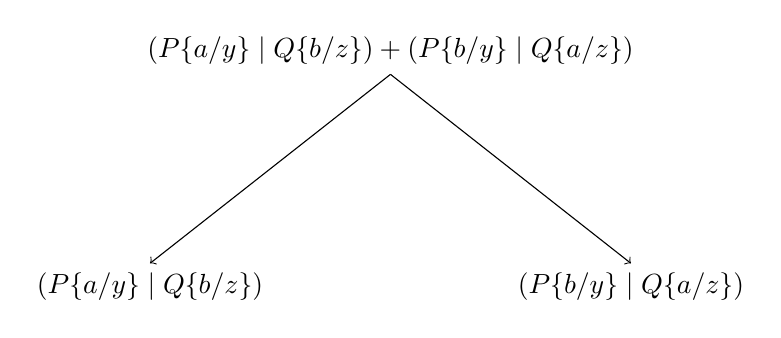
\begin{tikzpicture}[sibling distance=3cm,level distance=3cm]
    \Tree
    [.{$(\subst{P}{a}{y} \mid \subst{Q}{b}{z}) + (\subst{P}{b}{y} \mid \subst{Q}{a}{z})$}
    \edge[->]; {$(\subst{P}{a}{y} \mid \subst{Q}{b}{z})$}
    \edge[->]; {$(\subst{P}{b}{y} \mid \subst{Q}{a}{z})$}
    ]
  \end{tikzpicture}
\end{frame}

\begin{frame}{Local choice is not modular}
  \only<1>{%
    If we extend...
    \[
      \nu x.(x(y).P \mid x(z).Q \mid x[a].x[b].0)
    \]
    ...to...
    \[
      \nu x.(x(y).P \mid x(z).Q \mid x(w).R \mid x[a].x[b].x[c].0)
    \]
  }
  \only<2>{%
    Then we must extend...
    \[
      (\subst{P}{a}{y} \mid \subst{Q}{b}{z}) + (\subst{P}{b}{y} \mid \subst{Q}{a}{z})
    \]
    ...to...
    \[\!
      \begin{array}{cc}
        (\subst{P}{a}{y} \mid \subst{Q}{b}{z} \mid \subst{R}{c}{w}) &+ \\
        (\subst{P}{b}{y} \mid \subst{Q}{a}{z} \mid \subst{R}{c}{w}) &+ \\
        (\subst{P}{a}{y} \mid \subst{Q}{c}{z} \mid \subst{R}{b}{w}) &+ \\
        (\subst{P}{b}{y} \mid \subst{Q}{c}{z} \mid \subst{R}{a}{w}) &+ \\
        (\subst{P}{c}{y} \mid \subst{Q}{a}{z} \mid \subst{R}{b}{w}) &+ \\
        (\subst{P}{c}{y} \mid \subst{Q}{b}{z} \mid \subst{R}{a}{w})
      \end{array}
    \]
  }
\end{frame}


\end{document}